\chapter*{Layout en Stijl}
\chapterquote{De eerste eigenschap van stijl is helderheid.}{Aristoteles, Grieks filosoof (384 v.C. - 322 v.C.)}
Naast een cursus met een goeie inhoud, is ook de opmaak een belangrijk aspect. Om het leerproces zoveel mogelijk te bevorderen heeft de auteur volgende overwegingen gemaakt wat betreft de layout.
\paragraph{}
Alle pagina's zijn afdrukbaar met een zwart-wit printer. Dit drukt de eventuele kosten bij een afdruk van deze cursus. Bovendien verhoogt dit de leesbaarheid bij kleurenblindheid. Op het einde van de cursus staan enkele samenvattende schema's waar ook versies in kleur van beschikbaar zijn.
\paragraph{}
Deze cursus wordt ge\"illustreerd met talloze afbeeldingen. Deze zijn allemaal tot stand gekomen met het grafisch pakket Ti\textit{k}Z\footnote{TikZ ist kein Zeichenprogramm}. Alle afbeeldingen zijn bijgevolg vectorieel.
\begin{leftbar}
In elk hoofdstuk worden de technieken besproken aan de hand van een leidend voorbeeld. Tekst gerelateerd aan het leidend voorbeeld wordt zoals hier weergegeven met een zwarte rand. Indien de techniek in kwestie duidelijk is, mogen deze stukken overgeslagen worden.
\end{leftbar}
\paragraph{}
Belangrijke \termenlayout{terminologie} wordt in het vetjes zonder schreven\footnote{De zogenoemde ``pootjes'' die letters krijgen. (Engels: serifs)} gezet. Deze terminologie komt ook in de index achteraan de cursus. Deze index verwijst dus niet noodzakelijk naar de definities van de termen. Maar naar de pagina waar de term in kwestie voor het eerst voorkomt.
\begin{figure}[H]
\centering
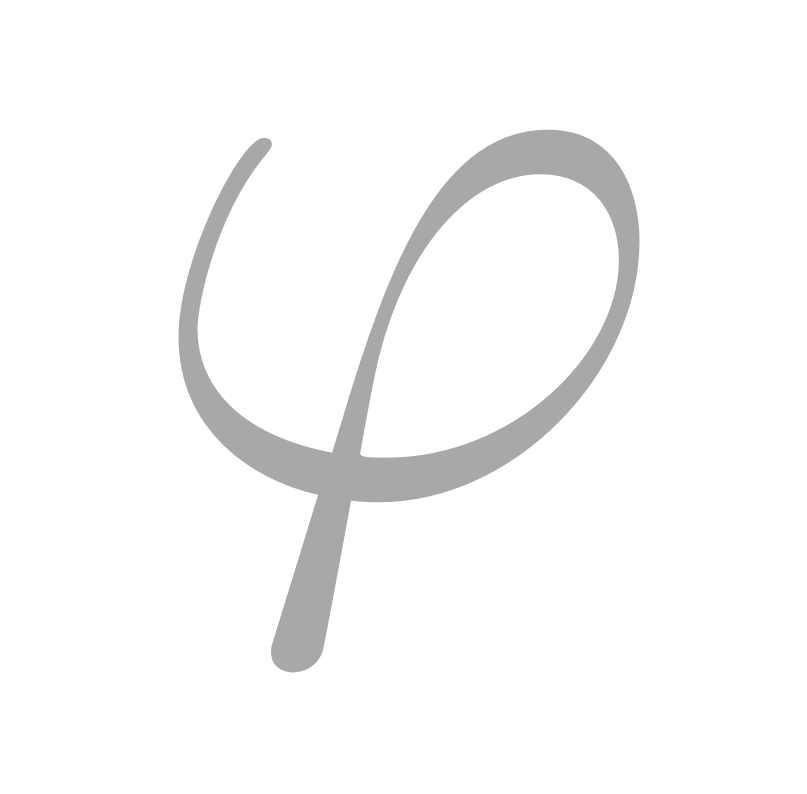
\begin{tikzpicture}
\draw[black!34] (0,0) node[scale=12]{\Huge{$\varphi$}};
\end{tikzpicture}
\end{figure}
